\section{What is OpenNMS?}
\emph{OpenNMS} is a network management platform to give you the ability to solve problems in the FCAPS\footnote{ISO Telecommunications Management Network model and framework for Fault, Configuration, Accounting, Performance and Security categories} categories. The application gives you access to the management data through a web interface. The \emph{OpenNMS} project is a collaboration of developers and network management specialists around the world, aiming to produce an open standard for a network management platform. The project aims to deliver a solution for all types of network management issues, massively scalable and feature-rich. The technology consists of a series of interrelated programs delivering various components for a cloud infrastructure solution.

\begin{figure}[h]
	\centering
	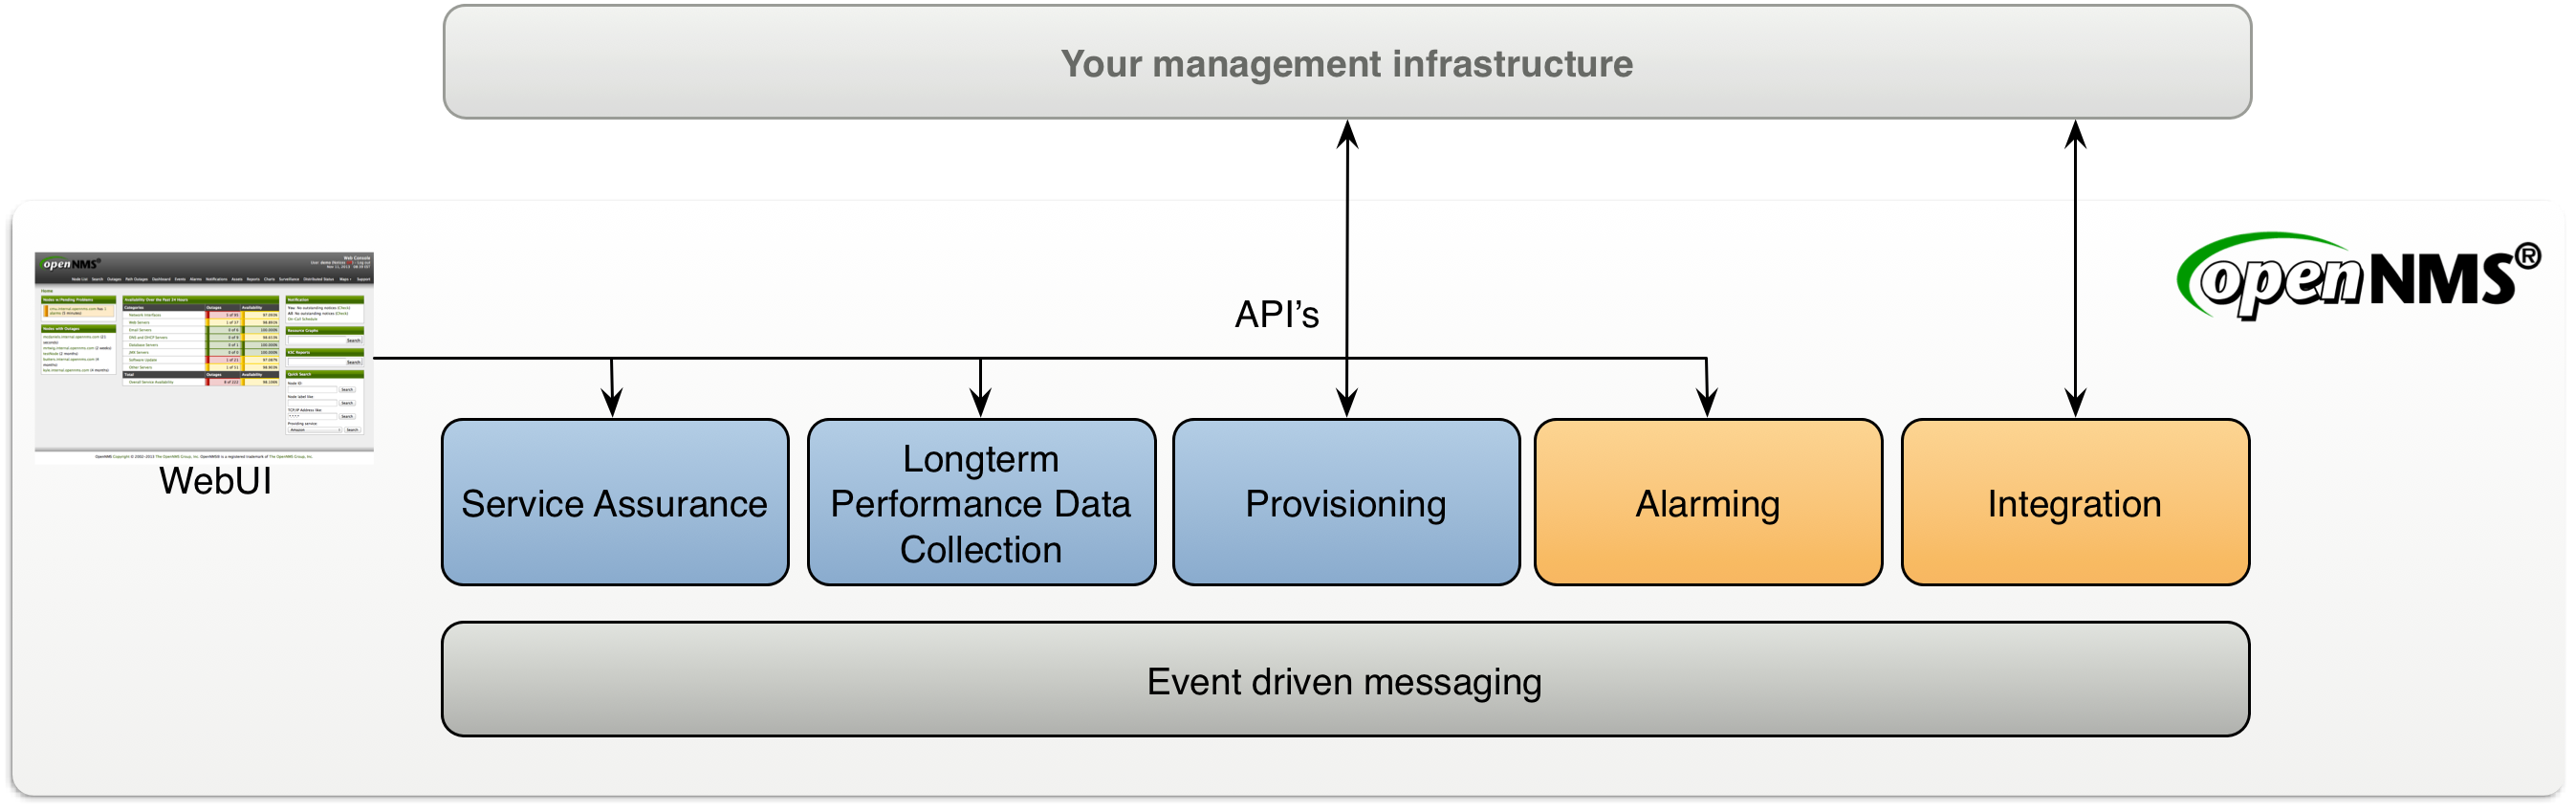
\includegraphics[width=1.0\textwidth]{images/opennms-principles.png}
	\caption{OpenNMS parts and principles}
	\label{fig:opennms-principles}
\end{figure}

The platform of \emph{OpenNMS} today provides a platform for long term performance data collection, service assurance and integration points for your management infrastructure.

\subsection{OpenNMS Principles}
\begin{itemize}
  \item Open development model: The entire code of \emph{OpenNMS} is freely available under GNU Public License Version 3\footnote{GPLv3 license: \url{http://www.gnu.org/copyleft/gpl.html}}.
  \item Open development process: Every year the development community holds a developers' conference to gather requirements and write specifications for the upcoming release.
  \item Open community: \emph{OpenNMS} is dedicated to producing a healthy, vibrant, and active developer and user community. Most decisions will be made using a ``lazy consensus'' model.
\end{itemize}

\subsection{OpenNMS Projects}
Network management has many different aspects of integration. Developing integrations against configuration management databases or vendor specific management architectures are common challenges. Otherwise there are also technology-specific topics, like different strategies to store and use time series data. All these different integrations projects are developed in the public git repository hosted at \url{https://www.github.com/opennms}.

\subsection{Release Process}
OpenNMS is currently on a \textbf{\textcolor{red}{???-month}} release cycle, which consists of \textbf{\textcolor{red}{x-many}} stages. Details on \textcolor{red}{\url{http://www.opennms.org/ReleaseCycle}}.

\subsubsection{Planning}
\textcolor{red}{Do we have a kind of a planning phase to decide which of the features come into a next release? Discussion, feedback to focus on the next release and lightweight spec writing.}

\subsubsection{Developers Conference}
\emph{The OpenNMS Group, Inc.} sponsors a developers' conference every year - \emph{DevJam}. This conference brings all core developers and community members together to work on the project. The conference is also used to discuss concepts around the project. We track \emph{DevJam} topics in our wiki, which can be found at \url{http://www.opennms.org/wiki/Dev-Jam}.

\subsubsection{JIRA}
\emph{OpenNMS} uses \emph{Atlassian JIRA} to track issues and for development planning. The development follows the agile \emph{Scrum} development process. Features are described as stories and will be developed in sprints. Details how we use \emph{JIRA} for the development process are documented at \textcolor{red}{\url{http://www.opennms.org/wiki/???}}

\subsubsection{Implementation}
The implementation stage is split into a number of milestone iterations. The work in progress is published in a feature branch, which should then be proposed for merging when ready. \textcolor{red}{Code is proposed several weeks before each milestone release date so that it can be reviewed in a timely manner. Is it that way?!}

\subsubsection{Quality Assurance}
For quality assurance we use \emph{Atlassian Bamboo} as continuous integration system\footnote{Open Source Licensed, https://www.atlassian.com/software/bamboo}. It is publicly available on \url{http://bamboo.internal.opennms.com:8085}. \emph{Bamboo} compiles and runs tests for feature- and master branches. Additionally, we use \emph{SonarQube}\footnote{SonarQube website: \url{http://www.sonarqube.org/}} for statistic code analysis. \textcolor{red}{\url{Where-is-the-URL-to-Sonar-I-dont-know?!}}. There are also branches intended to fix bugs, which means that they do not introduce new features. These branches are named after the \emph{JIRA} issue following the pattern NMS-\{issue-number\}. Builds are automatically triggered with committing to a feature- or master branch.

\subsubsection{Release}
Before a stable version is released, we have a release candidate freeze (RCF). This happens a \textbf{\textcolor{red}{x-days/weeks/months}} before an actual \textbf{\textcolor{red}{Release Day - do we have one?!}}. \emph{OpenNMS} releases are numbered using the \textbf{\textcolor{red}{YYYY.N time based scheme (our detailed scheme here, I have seen we changed with Bamboo our release scheme a bit.)}}. For example, \textbf{\textcolor{red}{an example follows here}}. The release is identified using a codename. Code names are \textbf{\textcolor{red}{Is there a pattern for our code names?}} \textbf{\textcolor{red}{Code names are chosen by people in the \emph{IRC} channel or whatever :) More details on \url{https://www.opennms.org/wiki/Release_Naming???}}}.

\subsection{Governance}
The \emph{OpenNMS} project is governed by \textbf{\textcolor{red}{your group here - OGPs + OpenNMS Group?!}}. \textbf{\textcolor{red}{Some ideas how OpenStack organized it, Foundation board of directors, technical committee, user comittee and a wiki page \url{http://wiki.openstack.org/Governance/Foundation/Bylaws}}}
